\documentclass[12pt]{article}
\title{Project Interviews}
\author{Bertagnoli Daniele 1903768 \\ Costantino Giuseppe 1677800 \\ Frascarelli Giacomo 1917888 \\ Guarino Marco 1895383}
\date{2023/2024}

\usepackage[left=2cm, right=2cm]{geometry}
\usepackage{amsmath}
\usepackage{graphicx}
\usepackage{subfig}
\usepackage{hyperref}

\begin{document}
\maketitle

\tableofcontents
\newpage

\section{Interviews}

\subsection{Questions}
These interviews were conducted to assess the viability of the project idea and serve as the initial stage of the need-finding process. The questions asked to the participants during the interview are:
\begin{enumerate}
    \item Have you experienced situations in which you or someone you know was in danger? (e.g., my father fell down and was not able to use the phone) If yes, what was the situation? Were you able to contact someone for help? Was it difficult, or were you able to alert someone easily?
    \item Would you install the application to alert contacts in an easy and fast way? Do you find this idea useful?
    \item Do you prefer to inform contacts through a phone call, SMS, or a notification? (Or other options)
    \item Would you install such an application to be informed about other contacts' emergencies? Why?
\end{enumerate}

\subsection{Answers}
The following rows contain the main content of each interview, 
highlighting the most significant contributions given by each participant:

\begin{enumerate}
    \item She said that once her grandmother had a medical emergency at 
    home, and she wasn't able to reach anyone for help because her phone 
    was out of reach. However, the grandmother is not able to use the 
    smartphone.
    
    \item He shared a story about a camping trip where one of his friends got 
    injured, and his phone fell several meters away from him. He started screaming 
    to ask for help, luckily, the other friends heard him. He said that he would 
    install that application only during particular periods of the year, such as when 
    he goes on holidays during summer. He prefers phone calls whenever possible.
    
    \item He mentioned a situation where a colleague experienced a severe allergic 
    reaction while he was alone at home. He was able to use the phone, but he 
    struggled to talk during the phone call with the ambulance operators. He said 
    that probably a method to alert family members in some ways with predefined 
    messages was probably the best thing in that situation because he had to alert 
    them several hours later when the crisis was gone. He told us that these 
    situations are not so common, so probably he wouldn't install such an application 
    as he prefers to be contacted via WhatsApp or SMS through that system.
    
    \item She told us about one situation in which she felt followed by someone. 
    Because she was very nervous, she had some difficulties quickly dialing her 
    mother's phone number on the phone. She stated that she would install the 
    application to feel safer when she comes back home during late hours of the day.
    
    \item He doesn't know anyone who experienced emergencies. He said that this is a 
    situation he has never thought about, but the application could be useful for his 
    grandma who lives alone and uses a smartphone. The interviewee prefers to be 
    informed via notifications.

    \item She said her mother fell to the ground in the evening, couldn't 
    get up, and couldn't call anyone. She would install an application that 
    could help herself and others in difficult situations. She 
    would like to be notified both by a call and by an SMS.
    
    \item She says she was alone in the middle of the night in Rome and felt 
    like someone was chasing her. So, she was on the phone the whole time 
    with her friend. She would like an application that can promptly assist 
    her in case of difficulty with a call. Additionally, she would install the 
    application to help other people in emergency situations.
    
    \item He has never experienced firsthand situations where he was in trouble 
    or where someone he knows alerted him in emergencies, but he would still 
    find an application for such purposes useful and would install it. 
    He would like to be notified, and to notify others, using all available 
    methods.
    
    \item He experienced a situation where his father had a heart attack 
    and fortunately managed to contact the ambulance but couldn't reach 
    his son, who only found out about the news after some time. So, he 
    would appreciate having the possibility of being contacted immediately. 
    He would thus install the application both in case he himself is in 
    danger and in case it's one of his parents. He would like to be 
    informed with a call and a notification of the location.
    
    \item She has never experienced situations of danger herself nor 
    secondhand where it was necessary to contact someone, but she would 
    appreciate an application that can alert others in a simplified way, 
    and to be alerted, in cases of danger and emergency. She would find it 
    useful to be notified in all available ways, through calls, SMS, and 
    notifications. She would install the application both for herself and 
    for friends or relatives.

    \item The interviewee had a nasty situation once while riding his bike. 
    He slipped while making a turn, and his smartphone flew out of his pocket. 
    Both his legs were stuck underneath the bike, and he was unable to move. 
    It wasn't until a good samaritan came by that he received medical 
    attention. He mentioned that had it been an isolated road with bad 
    weather, he could have easily died that day. He thinks calls are the 
    most effective way to get someone's attention, though a very loud 
    notification from the app could also work. He expressed interest in 
    using the app because his parents are getting older, and he would love 
    to keep an eye on them to be notified immediately in case of an 
    emergency.

    \item This person recounted an incident where she was trying to get her 
    grandfather to bed when he suddenly lost consciousness and fell on his 
    back. She immediately called the emergency number and got him escorted 
    to the hospital. She noted that her grandfather does not even have a 
    clamshell phone and is not keen on integrating technology into his 
    daily life. Thus, she does not think this idea could benefit her 
    family.

    \item She has had a few close calls while rock climbing. One time, she 
    fell and got stuck in a narrow crevice. A fellow climber nearby was able 
    to pull her out safely. This experience made her realize the importance 
    of a reliable emergency response system. She believes this idea could 
    benefit people with disabilities or mobility issues by providing an easy 
    way to alert contacts in case of an emergency. She thinks SMS messages 
    would be the most effective notification method to ensure the person 
    receiving the message is aware of the situation. She would definitely 
    install an app like this to keep an eye on loved ones who live far away, 
    understanding the importance of seniors having autonomy while still 
    having a safety net.

    \item He shared that his mum once fell down the stairs, which was quite 
    worrying for him and his brother. They managed to patch her up, and she 
    walked away with a minor scratch. While he finds the idea useful, he 
    does not trust technology enough. He worries about the phone's battery 
    running out, lack of signal, or a bug preventing a notification from 
    appearing. He prefers good old-fashioned phone calls and does not 
    believe apps can truly benefit daily life.

    \item The interviewee has never had a personal experience with danger 
    but has worked in emergency services for years. He has seen the impact 
    of timely interventions on people's lives, with one incident involving a 
    distress call from a lost hiker. He managed to locate and guide the 
    hiker back to safety, which highlighted the importance of having the 
    right tools and systems in place. He believes efficient communication is 
    crucial and views the app as a game-changer for staying connected and 
    getting help quickly. He thinks a combination of notifications and phone 
    calls would be most effective for alerting contacts in an emergency. 
    He would install the app to receive notifications about other contacts' 
    emergencies, believing in the importance of being connected and informed 
    to help each other, whether by providing support or offering a listening 
    ear.

    \item He recalled a time when his neighbor suffered a stroke while 
    gardening in the backyard. The neighbor's wife was inside the house 
    and unaware of the situation for several minutes. He believes an app 
    that could send alerts through loud notifications would be extremely 
    useful. He prefers SMS and notifications over calls, as they are less 
    intrusive but still effective. He would install the app to ensure his 
    family is informed in case of emergencies.

    \item She shared an incident where she was in a car accident and her 
    phone was damaged, making it impossible to call for help. A passerby 
    assisted her, but the experience made her realize the importance of 
    an emergency alert system. She would definitely install the app, 
    especially for her children who are often away at college. She 
    prefers notifications and SMS for their reliability and simplicity.

    \item He described a situation where his diabetic friend experienced 
    a severe hypoglycemic episode and couldn't reach his phone to call 
    for help. Another friend luckily noticed in time and assisted him. 
    He thinks the app would be beneficial, particularly for people with 
    medical conditions. He prefers notifications as the primary method 
    of alert. He would install the app to monitor his friend's condition 
    and ensure timely assistance.

    \item She mentioned an instance where her elderly father wandered 
    off and got lost while she was at work. It took hours to find him, 
    causing significant distress. She believes an app with GPS tracking 
    and emergency alerts could prevent such situations. She prefers phone 
    calls for immediate attention. She would install the app to keep 
    track of her father's whereabouts and ensure his safety.

    \item He recounted a time when he was hiking alone and twisted
    his ankle, making it difficult to move. His phone signal was weak, 
    and it took a long time to contact anyone for help. He believes an 
    emergency alert app that works in low-signal areas would be 
    invaluable. He prefers SMS for its reliability in such situations. 
    He would install the app for personal safety during solo outdoor 
    activities.

\end{enumerate}

\subsection{Interviews Analysis}
The interviews conducted provided valuable insights into the potential 
viability and usefulness of an emergency alert application. Participants 
shared a diverse range of experiences and opinions, highlighting both the
demand for such a solution and the considerations necessary for its 
successful implementation. There was a significant interest in the 
application among the participants, especially those who had encountered 
emergencies or had elderly family members living alone.

These intereviews underline a common theme: emergencies can occur 
unexpectedly, this highlights a clear need for an application 
that can facilitate quick and easy communication during such critical 
moments.

Preferences for notification methods varied among participants. 
Some preferred phone calls for their immediacy and effectiveness in 
grabbing attention during emergencies. Others favored SMS or app 
notifications, considering them more reliable and less intrusive. 

\section{Questionnaire}
For performing a more extended need-finding phase, we create a Google form 
with some questions to retrieve more information about our idea. The form 
is available at the following link: \url{https://forms.gle/1AnJ6wdFpiuWXPuFA}.

\subsection{Results}
We achieved a total of 80 answers and these are the results. As shown in 
\hyperref[fig:age]{Figure~\ref*{fig:age}}, more than $70\%$ of the partecipants
were having an age between 18 and 30 years old. 

\begin{figure}[ht]
    \centering
    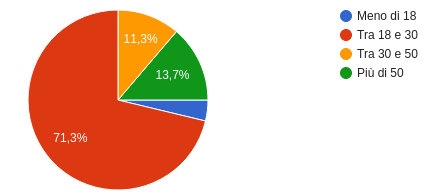
\includegraphics[width=.5\textwidth]{Images/age.png}
    \caption{Graph showing the partecipants' age.}
    \label{fig:age}
\end{figure}

From the second question, we can see how many participants have ever 
been in an emergency situation. $41.3\%$ have never experienced a 
critical situation, while $59.7\%$ have at least one experience. 
As we can see from \hyperref[fig:emergency_user]{Figure~\ref*{fig:emergency_user}},
only $16.3\%$ of the users were not able to alert someone during these 
situations. However, by taking a look at the next question, where the users 
described their experiences, we can see how most of these situations 
could generate so much panic that the user is not able to make quick 
decisions and thus even alerting someone using the phone can be difficult.

\begin{figure}[ht]
    \centering
    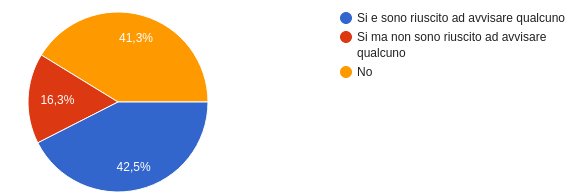
\includegraphics[width=.7\textwidth]{Images/emergency_user.png}
    \caption{Graph showing if the participants have ever experienced
    an emergency situation, and if they were able to alert someone.}
    \label{fig:emergency_user}
\end{figure}

The next two questions are very similar to the previous two. Nevertheless, 
in this case, the users were asked to answer if one of their acquaintances
has ever experienced one of these situations. Unlike the previous 
question, in this case $63.7\%$ of the participants answered 
"No" (\hyperref[fig:emergency_acquaintances]{Figure~\ref*{fig:emergency_acquaintances}}). 
If we look at the open answers, we can see how the experiences
are mostly similar to those described for personal experiences.

\begin{figure}[ht]
    \centering
    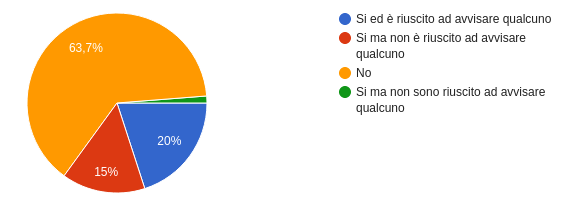
\includegraphics[width=.7\textwidth]{Images/emergency_acquaintances.png}
    \caption{Graph showing if the participants know someone who has ever 
    experienced an emergency situation, and if they were able to alert 
    someone.}
    \label{fig:emergency_acquaintances}
\end{figure}

The motivation most people give for using the app is that it makes the user save precious time.
The arguments being that if someone is injured, panic might prevent the user from making a swift
call to the emergency services.
Even worse, if someone is unable to use their cellphone due to severe injuries or fainting, users suggest
the app could help save their lives.
Other people argue that by intergrating the app with official first response services might result in
a quicker response time (\hyperref[fig:install_for_me]{Figure~\ref*{fig:install_for_me}}).

\begin{figure}[ht]
    \centering
    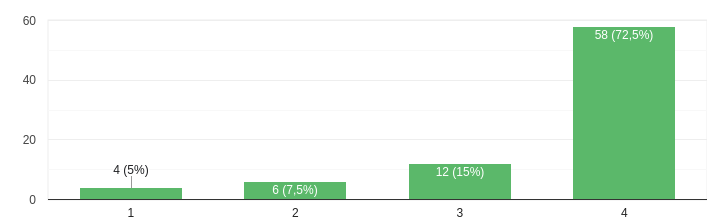
\includegraphics[width=.7\textwidth]{Images/install_for_me.png}
    \caption{Graph showing how the user will likely install the application
    for alerting their contacts.}
    \label{fig:install_for_me}
\end{figure}

A striking majority ($66.3\%$) of people would very surely install the applicaton (4)
followed by $21.3\%$ on option (3), $10.0\%$ on (2), which are not very convinced by the idea,
and lastly $2.5\%$ say they would not install the app.
Overall the response is positive and very encouraging.
(\hyperref[fig:install_for_others]{Figure~\ref*{fig:install_for_others}}).

\begin{figure}[ht]
    \centering
    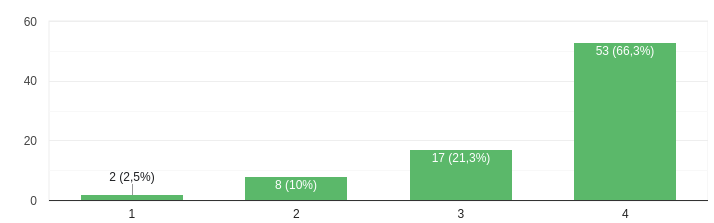
\includegraphics[width=.7\textwidth]{Images/install_for_others.png}
    \caption{Graph showing how the user will likely install the application
    for receiving alerts from their contacts.}
    \label{fig:install_for_others}
\end{figure}

More than half the people ($52.5\%$) would like to be informed by a notification
with relevant infos, followed by $30.0\%$ which would prefer to start an automatic
call to the person in potential danger, and lastly, with $16.3\%$ would prefer an SMS 
(\hyperref[fig:alert_me]{Figure~\ref*{fig:alert_me}}).

\begin{figure}[ht]
    \centering
    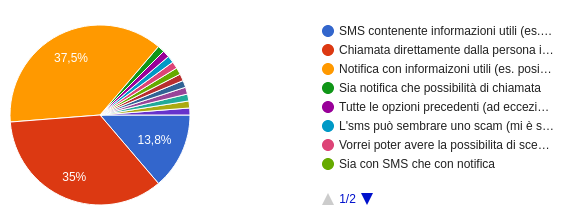
\includegraphics[width=.7\textwidth]{Images/alert_me.png}
    \caption{Graph showing how users want to be alerted.}
    \label{fig:alert_me}
\end{figure}

As for the mean through which people prefer to inform their contacts,
the majority ($37.5\%$) leans towards a notification with important informations.
Followed by an automatic call to a pre-determined contact ($35.0\%$) and lastly SMS 
to pre-determined contact (\hyperref[fig:alert_others]{Figure~\ref*{fig:alert_others}}).

\begin{figure}[ht]
    \centering
    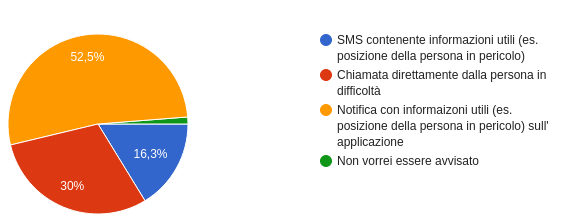
\includegraphics[width=.7\textwidth]{Images/alert_others.png}
    \caption{Graph showing how users want to alert their contacts.}
    \label{fig:alert_others}
\end{figure}

\section{Marvel Prototype}
As a first prototype, we decided to create a Marvel prototype, which can be tried 
at the following link: \url{https://marvelapp.com/prototype/fa2f7b8}. 
We conducted 12 tests with different users, trying to cover the widest 
age range possible. 

\subsection{Tasks}
During the tests, we asked each user to perform the following tasks:
\begin{enumerate}
    \item Try to activate the emergency mode. 
    \item Find settings and add a new contact.
    \item Modify the contact priority.
    \item Add a new notification method.
    \item Remove a detection.
\end{enumerate}

\subsection{Tests}
The following rows contain the main content of each test:
\begin{enumerate}
    \item The first user is a 55-year-old woman. The first task was completed 
    without hesitation. The second task required more time to be 
    executed as the user tried to uncheck one of the checked contacts. 
    However, due to a prototype limitation, this was not possible as we 
    didn't create enough screens to cover all possible combinations. 
    All the other tasks were performed easily. 

    \item The user is a 17-year-old boy. All tasks were executed 
    without problems. 

    \item The user is a 22-year-old woman. We repeated the test two times 
    due to a bug that caused a wrong screen to appear when tapping on the contacts after a particular sequence of actions. Once fixed, the tasks 
    were performed correctly. 
\end{enumerate}


\end{document}